\documentclass[12pt,a4paper]{article}
\usepackage[a4paper,margin=2.5cm]{geometry}
\usepackage{graphicx}
\usepackage{hyperref}
\usepackage{titlesec}
\usepackage{xcolor}
\usepackage{matlab-prettifier}
\usepackage{siunitx}
\usepackage{tikz}
\usepackage[version=4]{mhchem} 
\usepackage{comment}
\usepackage{listings}

\lstset{
	basicstyle=\ttfamily\small,
	showstringspaces=false,
	breaklines=true,
	frame=single,
}

\DeclareSIUnit{\Td}{Td}
\DeclareSIUnit{\atm}{atm}

\definecolor{dielcolor}{RGB}{171, 250, 186}
\definecolor{aircolor}{RGB}{205, 245, 253}
\definecolor{mygreen}{RGB}{67, 121, 57}

\makeatletter
\renewcommand{\boxed}[1]{\text{\fboxsep=.2em\fbox{\m@th$\displaystyle#1$}}}
\makeatother

\lstdefinelanguage{MyMatlab}{
	language     = Matlab,
	morekeywords = {
		if, else, elseif, end, for, while, switch, case, otherwise, break, return, function, global, persistent, try, catch, continue, parfor, spmd, classdef, properties, methods
	},
	deletekeywords = {
		linspace, plot, zeros, ones, mean, sum, length, size, eye, det, inv, sqrt, sin, cos, tan, pi, NaN
	}
}

\definecolor{matlab_string_color}{RGB}{167,9,245}
\definecolor{matlab_comment_color}{RGB}{0,128,19}
\lstdefinestyle{MatlabStyle}{
	language=MyMatlab,
	basicstyle=\ttfamily\small,
	keywordstyle=\color{blue},        % keywords
	stringstyle=\color{matlab_string_color},          % strings
	commentstyle=\color{matlab_comment_color}, % comments
	numbers=none,
	numberstyle=\tiny\color{gray},
	frame = none,
	showspaces=false,   % <-- this hides the ␣ symbol
	showtabs=false,     % optional
	showstringspaces=false,  % also hides spaces inside strings
	xleftmargin=0pt,     % remove left indentation
	columns=fullflexible,
	xrightmargin=0pt,   
	aboveskip=0pt,     % remove space above the listing
	belowskip=0pt,      % remove space below the listing  % optional: remove right margin
	morestring=[b]"                       % <-- double quotes as string delimiters
}

\newcommand{\matlabs}[1]{{\lstinline[style=MatlabStyle]!#1!}}

% --- Optional formatting ---
\hypersetup{
	colorlinks=true,
	linkcolor=blue,
	urlcolor=cyan
}

\newcommand{\seclink}[2]{%
	\begingroup
	\hypersetup{linkcolor=orange}%
	\hyperref[sec:#1]{\matlabs{#2}}%
	\endgroup
}


\titleformat{\section}{\large\bfseries\color{blue}}{\thesection}{1em}{}
\titleformat{\subsection}{\bfseries}{\thesubsection}{1em}{}

% --- Document info ---
\title{\textbf{Merlino2D User Manual}}
\author{Fabio Ragazzi}
\date{}

\begin{document}
	
	\maketitle
	\tableofcontents
	\newpage
	
	% ===============================
	\section{Introduction}
	
	Merlino2D solves time-dependent drift-diffusion-reaction equations on a 2D unstructured triangular mesh
	
	% ===============================
	\section{Installation}
	
	\subsection{Download}
	\href{https://github.com/PTL-Unibo/Merlino2D}{Here} you can download a ZIP folder containing the code. Alternatively, you can clone the repository with git:
	\begin{verbatim}
		> git clone https://github.com/PTL-Unibo/Merlino2D.git
	\end{verbatim}
	
	\subsection{Installation Steps}
	To use Merlino2D you need \href{https://it.mathworks.com/}{MATLAB} installed on your computer.
	You also need to install \href{https://gmsh.info/}{Gmsh} for mesh generation.
	The first time using Merlino2D it is necessary to run the script \textbf{Merlino2D\_startup.m}
	that is inside the \textbf{Code/} folder.
	By running this script, you will be asked to select the \textbf{gmsh.exe} executable that you should have previously installed on your computer.
	If the folder containing the project is moved to another location, you need to run \textbf{Merlino2D\_startup.m} again.
	
	\subsection{Verification}
	If the installation was successful, you can now run all the examples contained in the \textbf{cases/} folder. 
	We suggest that you start by running the script \textbf{c\_Diffusion.m}, which should not take a long time.
	By running that script, a Gmsh window containing a square divided into two half should appear. Closing that window the simulation will start and you should see the following text appearing in the Command Window:
	
	\matlabs{Generated Mesh}
	
	\matlabs{Initialization finished}
	
	\matlabs{Simulation finished}
	
	\matlabs{Deleted SquareCenterRefined.m}
	
	\noindent Finally, the following figure should appear:
	
	\begin{center}
		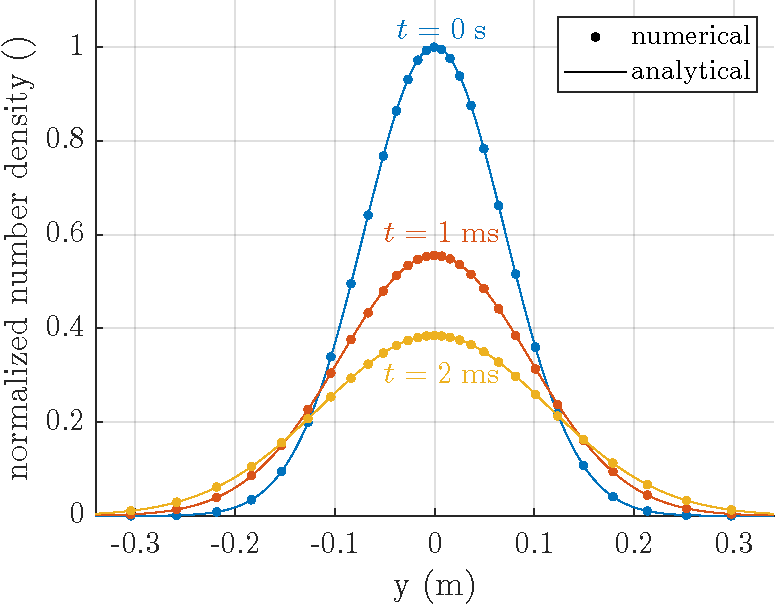
\includegraphics[width=8cm]{fig_diffusion.pdf}
	\end{center}
	
	\noindent If you see the above figure appearing without getting any errors, it means that you have successfully installed Merlino2D.
	
	
% ===============================
\section{Basic Workflow}

Every time you open MATLAB, to use the code you have to run the script \textbf{init.m}
that is inside the main folder. You can do it by selecting the file and pressing \textbf{F9}, or typing in the Command Window

\matlabs{>> init}

\noindent This will add to the MATLAB path the folder \textbf{Code/} that contains the code. 

\vspace{10pt}

\noindent The core of the code is the function \matlabs{Merlino2D}.
The syntax of the function is:

\matlabs{out = Merlino2D(opts,"key1",value1,"key2",value2,...);}

\noindent \matlabs{opts} is a structure that contains the input parameters for the simulation. 
Some parameters have a default value that can be found inside \textbf{DefaultMerlino2Dinput.m}.

\noindent The key-value arguments are optional and can be used to overwrite the parameters passed through \matlabs{opts}. 

\vspace{10pt}
\noindent \matlabs{out} is the unprocessed output structure that is given in input to the \matlabs{PostProcessing} function to obtain the post-processed output structure \matlabs{out\_pp}.

\matlabs{out\_pp = PostProcessing(out);}

\vspace{10pt}
\noindent \matlabs{out\_pp} can be used to plot the results using the \matlabs{Plot} function. 

\matlabs{Plot(out\_pp,"type",type\_value);}


\vspace{10pt}
\noindent To save the results of a simulation, use the \matlabs{Save} function.

\matlabs{Save(out\_pp,"my\_result.mat");}


\vspace{10pt}
\noindent To retrieve the results of a simulation that was previously saved, use the \matlabs{Load} function.

\matlabs{out\_pp = Load("my\_result.mat");}


\vspace{10pt}
\noindent It is also possible to export the results for visualization with Paraview using the \matlabs{ExportVTU} function. 

\matlabs{ExportVTU(out\_pp,"my\_results")}

\subsection{Post Processing}
There are two types of post processing, a lighter version and a more complete one.
To select which version to use, you can give to the function the string \matlabs{"light"} or \matlabs{"full"} as the second argument (\matlabs{"light"} is the default).

\matlabs{out\_pp = PostProcessing(out,"light");}

\matlabs{out\_pp = PostProcessing(out,"full");}

\noindent The lighter version will generate an output structure that contains:
\begin{itemize}
	\item the simulation time instants
	\item the number density of all the species at cells
	\item the surface charge density at the dielectric interface (if a dielectric material exists inside the domain)
	\item the electric potential at nodes
	\item the electric field at cells
	\item the charge density at cells
	\item the current over time computed with Sato's equation
	\item the applied voltage over time
	\item information about chemical species 
	\item information about the mesh
\end{itemize}

\noindent The full version adds to the previous list:
\begin{itemize}
	\item the electric field at faces
	\item the electric field at nodes
	\item the number density of all the species at nodes
	\item the charge density at nodes
	\item the flux density at faces
	\item the chemistry source term
	\item the current over time computed integrating the current density at electrodes
\end{itemize}


\subsection{Plot}
The \matlabs{Plot} function can plot several output quantities and will return the axes object \matlabs{ax}, containing the plot. It is possible to specify which type of plot to generate with the key-value argument \matlabs{"type"}.

\matlabs{ax = Plot(out\_pp,"type",<type\_value>);}


\noindent \matlabs{<type\_value>} needs to be a string. The available options are:
\begin{itemize}
\item \matlabs{"nc"}, to plot the species number density at cells
\item \matlabs{"nn"}, to plot the species number density at nodes
\item \matlabs{"rhoc"}, to plot the charge density at cells
\item \matlabs{"rhon"}, to plot the charge density at nodes
\item \matlabs{"phi"}, to plot the electric potential at nodes
\item \matlabs{"v-i"}, to plot the v-i characteristic
\item \matlabs{"Ec"}, to plot the electric field at cells
\item \matlabs{"|Ec|"}, to plot the electric field module at cells
\item \matlabs{"|En|"}, to plot the electric field module at nodes
\item \matlabs{"t-iv"}, to plot the current and voltage over time (in a single plot)
\item \matlabs{"t-Fx"}, to plot the force along x over time 
\item \matlabs{"fxc"}, to plot the force density along x at cells
\item \matlabs{"fxc\_log"}, to plot the force density along x at cells in log scale
\item \matlabs{"fxn"}, to plot the force density along x at nodes
\item \matlabs{"fxn\_log"}, to plot the force density along x at nodes in log scale
\item \matlabs{"rhon\_log"}, to plot the charge density at nodes in log scale
\item \matlabs{"sigma"}, to plot the surface charge density
\item \matlabs{"msh"}, to plot only the used mesh 
\end{itemize}
It is possible to pass to the \matlabs{Plot} function other key-value arguments. The available keys are:
\begin{itemize}
\item \matlabs{"ax"}: allows to pass the desired axes object to display the plot
\item \matlabs{"species\_index}: index of the chemical species to plot
\item \matlabs{"k"}: index of the time instant to display
\item \matlabs{"flip\_y"}: if equal to 1, plots also the symmetry of the domain with respect to the $x$-axis (for 2D color plots) and also \textbf{doubles the current}.
\item \matlabs{"log10\_zero\_val"}: for log scale plots sets the threshold under which everything is considered to be zero
\end{itemize}


\subsection{Save}
The \matlabs{Save} function needs a post processed output structure as input. 
Only the fields contained in the structure will be saved in a \textbf{.mat} file, so, be careful to the type of post processing that was performed (\matlabs{"light"} or \matlabs{"full"}).
The second input argument is an optional string that specifies the file where to save the results. If no second argument is given, the results will be saved with a string indicating the moment when the function was called, like: \matlabs{"2025\_12\_25\_12\_30\_00"}.

\matlabs{Save(out\_pp,"my\_result.mat");}

\matlabs{Save(out\_pp);}

\subsection{Load}
The \matlabs{Load} function takes as argument a string specifying the \textbf{.mat} file containing the results you want to load and returns the post processed output structure.

\matlabs{out\_pp = Load("my\_result.mat");}


	% ===============================
	\section{Numerical Identifiers of the Mesh}
	\label{sec:NemericalIdentifiers}
	\begin{center}
		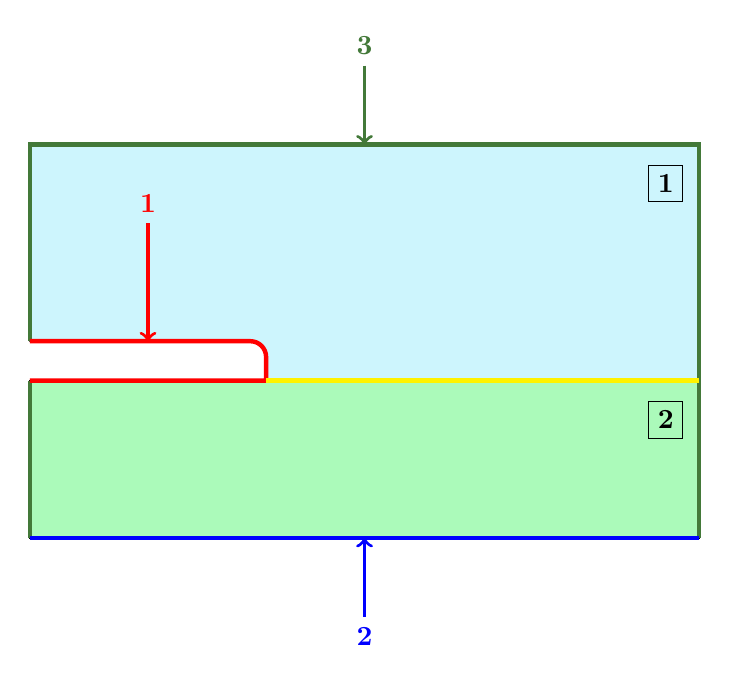
\begin{tikzpicture}
			\centering
			\pgfmathsetmacro{\scale}{1}
			\pgfmathsetmacro{\h}{5*\scale}
			\pgfmathsetmacro{\r}{0.2*\scale}
			\pgfmathsetmacro{\w}{8.5*\scale}
			\pgfmathsetmacro{\wdiel}{2*\scale}
			\pgfmathsetmacro{\welect}{0.5*\scale}
			\pgfmathsetmacro{\lelect}{3*\scale}
			\draw[fill=dielcolor] (0,0) rectangle ++(\w,\wdiel);
			\draw[fill=aircolor] (\lelect,\wdiel) -- (\lelect,\wdiel+\welect-\r) arc[start angle=0, end angle=90, radius=\r] -- (0,\wdiel+\welect) -- (0,\h) -- (\w,\h) -- (\w,\wdiel) -- cycle;
			\draw[mygreen,ultra thick] (0,0) -- (0,\wdiel);
			\draw[mygreen,ultra thick] (0,\wdiel+\welect) -- (0,\h) -- (\w,\h) -- (\w,0);    
			\draw[red,ultra thick] (0,\wdiel) -- (\lelect,\wdiel) -- (\lelect,\wdiel+\welect-\r) arc[start angle=0, end angle=90, radius=\r] -- (0,\wdiel+\welect);
			\draw[blue,ultra thick] (0,0) -- (\w,0);
			\draw[->, very thick, mygreen] (\w*0.5,6*\scale) -- (\w*0.5,\h)
			node[pos=0,above]{\textbf{3}};
			\draw[->, very thick, blue] (\w*0.5,-1*\scale) -- (\w*0.5,0)
			node[pos=0,below]{\textbf{2}};
			\draw[->, very thick, red] (\lelect*0.5,0.8*\h) -- (\lelect*0.5,\wdiel+\welect)
			node[pos=0,above]{\textbf{1}};
			\node[draw] at (\w*0.95,\h*0.3) {\textbf{2}};
			\node[draw] at (\w*0.95,\h*0.9) {\textbf{1}};
			\draw[yellow,ultra thick] (\lelect,\wdiel) -- (\w,\wdiel);
		\end{tikzpicture}
	\end{center}
	Let us consider an example domain composed of a \colorbox{aircolor}{gas region} (above the yellow line) and a \colorbox{dielcolor}{solid dielectric region} (below the yellow line), separated by a dielectric interface (the yellow line). Suppose that the user intends to apply three different boundary conditions to the regions highlighted in \textcolor{red}{red}, \textcolor{blue}{blue}, and \textcolor{mygreen}{green}.
	
	When generating a mesh to use in Merlino2D, each external boundary where a distinct boundary condition is required must be assigned a unique numerical identifier. For instance, in this case, the three external regions can be labeled with the identifiers \textcolor{red}{1}, \textcolor{blue}{2}, and \textcolor{mygreen}{3}, respectively. These identifiers are defined in the \textbf{.geo} file using the \matlabs{Physical Curve} command.
	Similarly, each subdomain corresponding to a different relative permittivity value $\varepsilon_r$ must be assigned a unique identifier. In the present example, the gas and solid dielectric regions are labeled as \colorbox{aircolor}{1} and \colorbox{dielcolor}{2}, respectively. These identifiers are defined in the \textbf{.geo} file using the \matlabs{Physical Surface} command.
	
	Note that \textbf{Merlino2D treats as gas only regions with a surface identifier equal to 1}, whereas all regions assigned a numerical identifier greater than 1 are interpreted as solid dielectric materials.
	Note also that \textbf{Merlino2D identifies as dielectric interfaces only lines assigned a numerical identifier greater than or equal to 8854} \footnote{This apparently random number actually corresponds to the first four digits of the vacuum permittivity $\varepsilon_0 = \SI{8.8541878188e-12}{\farad\per\meter}$.}.
	For this reason, in the \textbf{.geo} file, the yellow line can be labeled, for example, with the identifier 8888 using the \matlabs{Physical Curve} command.
	
	In general, a mesh provided as input to Merlino2D includes identifiers for the external boundaries, hereafter referred to as \textbf{BoundaryIDs} (\textcolor{red}{1}, \textcolor{blue}{2}, and \textcolor{mygreen}{3} in the previous example), as well as identifiers for the subdomains, hereafter referred to as \textbf{SurfaceIDs} (\colorbox{aircolor}{1} and \colorbox{dielcolor}{2} in the previous example).
	
	\section{Species Database}
	All species used in a simulation—whether defined within the \matlabs{reactions} variable of the kinetic scheme specified by \seclink{chemicalmodel}{CHEMICAL\_MODEL}, or listed in the \seclink{speciesnochem}{SPECIES\_NO\_CHEM} input parameter—must be included in the \textbf{species\_database.csv} file located in the \textbf{data/} folder.
	This file is a comma-separated values (CSV) file containing three columns. 
	\begin{itemize}
	\item The first column lists the names of the species. Every species name used in the \matlabs{reactions} variable or appearing in \seclink{speciesnochem}{SPECIES\_NO\_CHEM} must be present in this first column of \textbf{species\_database.csv}. 
	
	\item The second column contains the mass of the species, expressed in \unit{\kilogram}. 
	
	\item The third column contains the charge of the species. 
	\end{itemize}
	
	\lstinputlisting{../data/species_database.csv}
	New species that the user wants to consider in a simulation must be added here.
	
	\section{Input Parameters}
	
	\subsection{MSH}
	\label{sec:msh}
	This parameter is a string used to specify the mesh file.
	For example, if you have created a file \textbf{My\_mesh.geo} with Gmsh, and you want to run a simulation on that mesh, you must first of all put the file inside the \textbf{geo/} folder.
	To tell the code that you want to run the simulation on that mesh, you have to set the \seclink{msh}{MSH} parameter to the name of the \textbf{.geo} file:
	
	\matlabs{opts.MSH = "My\_mesh";}
	
	\noindent Note that you must have at the end of the \textbf{.geo} file a line that saves the mesh in the MATLAB format. So, considering the previous example, at the end of the file \textbf{My\_mesh.geo} you must have the line: 
	
	{\small \texttt{Save "My\_mesh.m";}}
	
	\subsection{MSH\_PARAMETERS}
	\label{sec:mshparam}
	This parameter is a struct that contains in its fields extra inputs that you might want to pass to a parametric mesh.
	It is indeed possible to create \textbf{.geo} files that accept parameters from command line. 
	For example you can create a mesh file that generates a rectangle, taking the width \textbf{W} and height \textbf{H} from command line.
	Supposing you want to pass \textbf{W} = 2 and \textbf{H} = 1 to the mesh file (that you have specified with the \seclink{msh}{MSH} parameter), you can do it with this syntax:
	
	\matlabs{opts.MSH\_PARAMETERS.W = 2;}
	
	\matlabs{opts.MSH\_PARAMETERS.H = 1;}
	
	\subsection{EPSR\_VAL}
	\label{sec:epsrval}
	This parameter is used to set the value of the relative dielectric permittivity $\varepsilon_r$ in each region of the simulation domain. \seclink{epsrval}{EPSR\_VAL} must be a \textbf{column} vector with as many elements as there are SurfaceIDs (see Section \ref{sec:NemericalIdentifiers}). Referring to the example in \ref{sec:NemericalIdentifiers}, if you wish to set $\varepsilon_r$ to 1 and 4 in the \colorbox{aircolor}{1} and \colorbox{dielcolor}{2} regions, respectively, you should set
	
	\matlabs{opts.EPSR\_VAL = [1; 4];}
	
	\subsection{BCEL\_FLAG}
	\label{sec:bcelflag}
	This parameter specifies the type of boundary conditions applied to the electric potential. \seclink{bcelflag}{BCEL\_FLAG} must be a \textbf{column} vector containing as many elements as there are BoundaryIDs (see Section \ref{sec:NemericalIdentifiers}). Each element of the vector can be set to 0, corresponding to a Dirichlet boundary condition at the associated external boundary, or 1, corresponding to a zero Neumann condition. Referring to the example in \ref{sec:NemericalIdentifiers}, if you want to apply a Dirichlet boundary condition at external boundaries \textcolor{red}{1} and \textcolor{blue}{2}, and a zero Neumann condition at external boundary \textcolor{mygreen}{3}, you should set
	
	\matlabs{opts.BCEL\_FLAG = [0; 0; 1];}
	
	\subsection{BCEL\_VAL}
	\label{sec:bcelval}
	This parameters is used to set the value of the electric potential at those boundaries where a Dirichlet condition is used. \seclink{bcelval}{BCEL\_VAL} must be a \textbf{column} vector containing as many elements as there are BoundaryIDs (see Section \ref{sec:NemericalIdentifiers}). Each element corresponding to a boundary with a Dirichlet condition should contain the value of the electric potential imposed at that boundary \textbf{normalized by \seclink{vapplied}{V\_APPLIED}}. All the other elements of the vector (corresponding to zero Neumann boundaries) should be set to 0. Referring to the example in \ref{sec:NemericalIdentifiers}, if you want to apply an electric potential equal to half \matlabs{V\_APPLIED} at the boundary \textcolor{red}{1} and set the potential at boundary \textcolor{blue}{2} to 0, you should set
	
	\matlabs{opts.BCEL\_VAL = [0.5; 0; 0];}
	
	\subsection{V\_APPLIED}
	\label{sec:vapplied}
	This parameter is a function handle used to specify the applied voltage between the electrodes, as a function of time. The user can define any custom function.
	
	\matlabs{opts.V\_APPLIED = @(t) 100*cos(2*pi*50*t + pi/4);}
	
	\matlabs{opts.V\_APPLIED = @(t) 20*(t-1e-9);}
	
	\matlabs{opts.V\_APPLIED = @(t) 20e3;}
	
	\noindent For DC discharges, it was observed that applying from the start the steady-state voltage may lead to failure of the time-integration solver. Gradually increasing the voltage until reaching the desired value often solved the problem. For this reason, some functions that implement this gradual increase of the voltage are provided in Merlino2D:  
	
	\begin{itemize}
		\item \matlabs{LinRamp}
		\item \matlabs{LogRamp}
		\item \matlabs{StairRamp} (particularly useful for obtaining the I-V characteristic of a corona discharge)
	\end{itemize}
	
	\subsection{BC\_FLAG}
	\label{sec:bcflag}
	This parameter is used to specify the type of boundary condition for the species conservation equation.
	\seclink{bcflag}{BC\_FLAG} must be a cell array with two columns. 
	
	In the first column, you should put strings containing the names of the species considered for the simulation. If \seclink{chemicalmodel}{CHEMICAL\_MODEL} was set to a \textbf{.m} script, the species must be the ones appearing in the \matlabs{reactions} defined inside the script.
	If \seclink{chemicalmodel}{CHEMICAL\_MODEL} was set to \matlabs{"Off"}, the species must be the ones specified in \seclink{speciesnochem}{SPECIES\_NO\_CHEM}. Note that all the species used must be defined inside the file \textbf{species\_database.csv} contained in the \textbf{data/} folder.
	
	Each element of the second column must be a row cell array with as many elements as there are BoundaryIDs (see Section \ref{sec:NemericalIdentifiers}). Each one of these cell arrays will be used to set the boundary condition for the continuity equation of the species that appears at the corresponding position in the first column of \seclink{bcflag}{BC\_FLAG}. 
	The $ith$ element of one of these cell arrays must be a string specifying the type of boundary condition to be applied at the $ith$ boundary.
	The available types of boundary conditions are (see the paper for details):
	\begin{itemize}
		\item \matlabs{"Dirichlet"}
		\item \matlabs{"Flux"}
		\item \matlabs{"FreeDriftFlow"}
		\item \matlabs{"GorinLike"}
	\end{itemize}
	For instance, considering a mesh with 3 BoundaryIDs and 2 species (\matlabs{"e"} and \matlabs{"N2+"}, that must be defined inside \textbf{species\_database.csv}), you could set
	
	\matlabs{opts.BC\_FLAG = \{}
	
	\hspace{40pt} \matlabs{"e", \{"GorinLike", "Flux", "Dirichlet"\};}
	
	\hspace{40pt} \matlabs{"N2+", \{"GorinLike", "FreeDriftFlow", "Flux"\}\};}

	
	\subsection{BC\_VAL}
	\label{sec:bcval}
	This parameter is used to specify the value of boundary conditions for the species continuity equation.
	\seclink{bcval}{BC\_VAL} must be a cell array with two columns.
	
	In the first column, you should put strings containing the names of the species considered for the simulation. If \seclink{chemicalmodel}{CHEMICAL\_MODEL} was set to a \textbf{.m} script, the species must be the ones appearing in the \matlabs{reactions} defined inside the script.
	If \seclink{chemicalmodel}{CHEMICAL\_MODEL} was set to \matlabs{"Off"}, the species must be the ones specified in \seclink{speciesnochem}{SPECIES\_NO\_CHEM}. Note that all the species used must be defined inside the file \textbf{species\_database.csv} contained in the \textbf{data/} folder.

	Each element of the second column must be a row cell array with as many elements as there are BoundaryIDs (see Section \ref{sec:NemericalIdentifiers}). Each one of these cell arrays will be used to set the boundary condition value for the continuity equation of the species that appears at the corresponding position in the first column of \seclink{bcval}{BC\_VAL}. 
	The $ith$ element of these cell arrays can be an anonymous function (if you wish to set a time-dependent value) or a double (if you wish to set a constant value), specifying the boundary condition to be applied at the $ith$ boundary.
	Note that \seclink{bcval}{BC\_VAL} is complementary to \seclink{bcflag}{BC\_FLAG}, and only boundary conditions of type \matlabs{"Dirichlet"} or \matlabs{"Flux"} require a value. Therefore, \seclink{bcval}{BC\_VAL} contains the desired value of number density (in \unit{\per\cubic\meter}) if a \matlabs{"Dirichlet"} condition was selected, and the desired value of flux density (in \unit{\per\square\meter\per\second}) if a \matlabs{"Flux"} condition was selected. For boundaries that were associated to \matlabs{"GorinLike"} or \matlabs{"FreeDriftFlow"} conditions, the corresponding value specified in \seclink{bcval}{BC\_VAL} will be ignored (but you must place some value anyway).
	
	For example, considering the case of a mesh with 3 BoundaryIDs and 2 species, where you previously set
	
	\matlabs{opts.BC\_FLAG = \{}

	\hspace{40pt} \matlabs{"e", \{"GorinLike", "Flux", "Dirichlet"\};}
	
	\hspace{40pt} \matlabs{"N2+", \{"GorinLike", "FreeDriftFlow", "Flux"\}\};}
	
	\noindent you could set
	
	\matlabs{opts.BC\_VAL = \{}
	
	\hspace{40pt} \matlabs{"N2+", \{NaN, NaN, @(t)t\^2\};}
	
	\hspace{40pt} \matlabs{"e", \{NaN, @(t)1e10*t, 1e15\}\};}
		
	\noindent With this combination of parameters you are imposing a constant number density of \SI{1e5}{\per\cubic\meter} for the species \matlabs{"e"} at the third boundary, and a time-dependent expression for computing the flux of \matlabs{"e"} at the second boundary and of \matlabs{"N2+"} at the third boundary. Notice that \matlabs{NaN} have been placed in \seclink{bcval}{BC\_VAL} at positions corresponding to \matlabs{"GorinLike"} and \matlabs{"FreeDriftFlow"} flags. This was done to highlight that, for those species and boundaries where a \matlabs{"GorinLike"} or a \matlabs{"FreeDriftFlux"} condition has been used, the value inserted in the corresponding position of \seclink{bcval}{BC\_VAL} will be completely ignored.
	
	
	
	
	\subsection{TIME\_INSTANTS}
	\label{sec:timeinst}
	This parameter is a vector containing the time instants at which the solution is desired. The first value of the vector corresponds to the starting time of the simulation, and the last value of the vector tells the solver when to stop integration. 
	If a vector with only two elements is provided, the solver will output all the steps that have been internally performed. Be careful in this case, because this might result in a lot of output time steps, that can quickly fill the memory, especially when meshes with a large number of triangles are used.
	
	\matlabs{opts.TIME\_INSTANTS = linspace(0,1e-6,100);}
	
	\matlabs{opts.TIME\_INSTANTS = [0, 1e-6];}
	
	\subsection{INITIAL\_CONDITION}
	\label{sec:initial}
	This parameter is used to specify the initial condition for the species number density. There are three types of use for this parameter:
	\begin{itemize}
		\item Uniform number density 
		\item Load from previous simulation
		\item Gaussian distribution (only when \seclink{chemicalmodel}{CHEMICAL\_MODEL} = \matlabs{"Off"})
	\end{itemize}
	
	\paragraph{Uniform number density}
	If you wish to assign a uniform number density to each species across the entire domain, set \seclink{initial}{INITIAL\_CONDITION} to a cell array with two columns.
	
	In the first column, you should put strings containing the names of the species considered for the simulation. If \seclink{chemicalmodel}{CHEMICAL\_MODEL} was set to a \textbf{.m} script, the species must be the ones appearing in the \matlabs{reactions} defined inside the script.
	If \seclink{chemicalmodel}{CHEMICAL\_MODEL} was set to \matlabs{"Off"}, the species must be the ones specified in \seclink{speciesnochem}{SPECIES\_NO\_CHEM}. Note that all the species used must be defined inside the file \textbf{species\_database.csv} contained in the \textbf{data/} folder.
	
	In the second column, you should put the desired uniform number densities in \unit{\per\cubic\meter}. Each of these values will be associated to the corresponding species in the first column. 
	
	\matlabs{opts.INITIAL\_CONDITION = \{}
	
	\hspace{40pt} \matlabs{"e", 1e10;}
	
	\hspace{40pt} \matlabs{"N2+", 1e12;}
	
	\hspace{40pt} \matlabs{"O2+", 1e13;}
	
	\hspace{40pt} \matlabs{"N2", 1e25\};}
	
	\paragraph{Load from previous simulation}
	If you wish to start a simulation using the number density distribution obtained at the end of a previous run, set \seclink{initial}{INITIAL\_CONDITION} to a string containing the absolute path of the saved results file (the \textbf{.mat} file generated by the \matlabs{Save} command). For example:
	
	\matlabs{opts.INITIAL\_CONDITION = "C:/Users/JohnSmith/Merlino2D/Results/test.mat";}
	
	\noindent Alternatively, you can specify a relative path; however, this approach is less reliable, as it may fail depending on the working directory at the time Merlino2D is executed.
	For instance, if the simulation is launched from the main Merlino2D folder, the following command is also valid:
	
	\matlabs{opts.INITIAL\_CONDITION = "Results/test.mat";}
	
	\noindent For this usage, the mesh should be the same of the previous simulation, as well as the species.
	
	\paragraph{Gaussian distribution}
	This option is available only when \seclink{chemicalmodel}{CHEMICAL\_MODEL} is set to \matlabs{"Off"}.
	In this case, if you wish to assign to each species a two-dimensional Gaussian distribution, set \seclink{initial}{INITIAL\_CONDITION} to a struct with fields
	\begin{itemize}
		\item A
		\item B
		\item x0
		\item y0
		\item sigma\_x
		\item sigma\_y
	\end{itemize}
	each of them being a vector with as many elements as the number of species contained in \seclink{speciesnochem}{SPECIES\_NO\_CHEM}. This will generate for the \textbf{ith} species contained in \seclink{speciesnochem}{SPECIES\_NO\_CHEM} a number density distribution
	\[
	n_i(x,y) = \boldsymbol{\mathrm{A}}[i] \, \mathrm{exp}\left(-\left(\frac{(x-\boldsymbol{\mathrm{x0}}[i])^2}{\boldsymbol{\mathrm{sigma\_x}}[i]} + \frac{(y-\boldsymbol{\mathrm{y0}}[i])^2}{\boldsymbol{\mathrm{sigma\_y}}[i]}\right)\right) + \boldsymbol{\mathrm{B}}[i].
	\]
	where the value of the parameters A, B, x0, y0, sigma\_x and sigma\_y is taken from the corresponding \textbf{i} element of the array. Note that the order of the numbers inside these arrays is important. For example you could set
	
	\matlabs{opts.INITIAL\_CONDITION.A = [1e10, 1e11];}
	
	\matlabs{opts.INITIAL\_CONDITION.B = [1e5, 0];}
	
	\matlabs{opts.INITIAL\_CONDITION.x0 = [1e-2, 0];}
	
	\matlabs{opts.INITIAL\_CONDITION.y0 = [1e-2, 1e-1];}
	
	\matlabs{opts.INITIAL\_CONDITION.sigma\_x = [1e-3, 1e-3];}
	
	\matlabs{opts.INITIAL\_CONDITION.sigms\_y = [1e-2, 1e-2];}
	
	\subsection{MU}
	\label{sec:mu}
	This parameter is used to set the mobilities of the species, in \unit{\square\meter\per\volt\per\second}. \seclink{mu}{MU} must be a cell array with two columns.
	
	In the first column, you should put strings containing the names of the species considered for the simulation. If \seclink{chemicalmodel}{CHEMICAL\_MODEL} was set to a \textbf{.m} script, the species must be the ones appearing in the \matlabs{reactions} defined inside the script.
	If \seclink{chemicalmodel}{CHEMICAL\_MODEL} was set to \matlabs{"Off"}, the species must be the ones specified in \seclink{speciesnochem}{SPECIES\_NO\_CHEM}. Note that all the species used must be defined inside the file \textbf{species\_database.csv} contained in the \textbf{data/} folder.
	
	The elements in the second column will be used to determine the mobility of the corresponding species in the first column. Each element of the second column can be a number (if you wish to set a constant and uniform mobility) or a string. You should use a string to write an expression that will be used to compute the mobility.
	In the string, you can use any valid Matlab syntax to combine the available standard variables \textbf{E}, \textbf{Te}, \textbf{T} and \textbf{Ngas}, which correspond to the electric field in \unit{\Td}, the electron temperature in \unit{\electronvolt}, the gas temperature in K, and the gas density in \unit{\per\cubic\meter}, respectively. Note that the first three are arrays with as many elements as domain points, while the last one is a scalar. For example, you can set
	
	\matlabs{opts.MU = \{}
	
	\hspace{40pt} \matlabs{"e", 0.001;}
	
	\hspace{40pt} \matlabs{"O2-","exp(E/120)*T\^(-0.5)";} 
		
	\hspace{40pt} \matlabs{"O4+", "Ngas*max(log(T),Te\^(-0.2))"\};}
	
	\noindent to have a constant mobility for the species \matlabs{"e"} and a mobility that is computed as a function of \textbf{E}, \textbf{Te}, \textbf{T}, and \textbf{Ngas} for the species \matlabs{"O2-"} and \matlabs{"O4+"}.
	
	Inside the string expressions, you can also use \textbf{.csv} files contained inside the \textbf{data/} folder to define new variables (called csv variables).
	For example, suppose that you have obtained a relation between the reduced mobility and the reduced electric field, and that you have stored that relation inside a file \textbf{my\_reduced\_Mobility.csv}, where the first column contains the values of the reduced electric field, and the second column contains the values of the reduced mobility. In this case, you can set
	
	\matlabs{opts.MU = \{}
	
	\hspace{40pt} \matlabs{"O2-","exp(E/120)*T\^(-0.5)";} 
	
	\hspace{40pt} \matlabs{"e", 0.001;}
	
	\hspace{40pt} \matlabs{"O4+", "my\_reduced\_Mobility(E)/Ngas"\};}
	
	\noindent to use the relation contained inside the \textbf{.csv} file to compute the mobility of \matlabs{"O4+"}. Note that csv variables can be combined with standard variables, as you can see from the fact that \matlabs{"my\_reduced\_Mobility"} is divided by the gas density \matlabs{"Ngas"}. It is also possible to combine different csv variables inside a string expression.
	
	Also, note that you must specify the dependence of the csv variable from one of the four standard variables. For instance, in the above example, \matlabs{"(E)"} was added after the name of the csv variable to indicate that in the first column of the \textbf{.csv} file are stored the values of reduced electric field. If you wish to define a csv variable that depends on the value of the electron temperature, you must add \matlabs{"(Te)"} after the name of the variable, like 
	
	\matlabs{opts.MU = \{}
	
	\hspace{40pt} \matlabs{"O2-","exp(E/120)*T\^(-0.5)";} 
	
	\hspace{40pt} \matlabs{"e", 0.001;}
	
	\hspace{40pt} \matlabs{"O4+", "my\_mob\_as\_func\_of\_Te(Te)"\};}
	
	\noindent In case you set a value for \seclink{lokiinput}{LOKI\_INPUT}, additional variables (called loki variables) will be available. These are: \textbf{Loki\_D}, \textbf{Loki\_mu}, \textbf{Loki\_alpha}, \textbf{Loki\_eta}. They represent the reduced electron diffusion coefficient, the reduced electron mobility, the reduced Townsned ionization coefficient, and the reduced attachment coefficient, respectively.
	These variables work in the same way of csv variables, but are available without the need to define any \textbf{.csv} file, since they are obtained from the LoKI-B simulation specified with \seclink{lokiinput}{LOKI\_INPUT}. In addition, these variables are all dependent on the reduced electric field, which means that they must always appear inside a string expression as \matlabs{Loki\_D(E)}, \matlabs{Loki\_mu(E)}, \matlabs{Loki\_alpha(E)}, and \matlabs{Loki\_eta(E)}. For example, you could set
	
	\matlabs{opts.MU = \{}
	
	\hspace{40pt} \matlabs{"e", "Loki\_mu(E)/Ngas";} 
	
	\hspace{40pt} \matlabs{"N2+", 1e-4;}
	
	\hspace{40pt} \matlabs{"O-", "exp(E/120)*T\^(-0.5)"\};}
	
	\subsection{D}
	\label{sec:d}
	This parameter is used to set the diffusion coefficient of the species, in \unit{\square\meter\per\second}. \seclink{D}{D} must be a cell array with two columns.
	
	In the first column, you should put strings containing the names of the species considered for the simulation. If \seclink{chemicalmodel}{CHEMICAL\_MODEL} was set to a \textbf{.m} script, the species must be the ones appearing in the \matlabs{reactions} defined inside the script.
	If \seclink{chemicalmodel}{CHEMICAL\_MODEL} was set to \matlabs{"Off"}, the species must be the ones specified in \seclink{speciesnochem}{SPECIES\_NO\_CHEM}. Note that all the species used must be defined inside the file \textbf{species\_database.csv} contained in the \textbf{data/} folder.
	
	The elements in the second column will be used to determine the diffusion coefficient of the corresponding species in the first column. Each element of the second column can be a number (if you wish to set a constant and uniform value for the diffusion coefficient) or a string (if you wish to define an expression that will be used to compute the value of the diffusion coefficient). The exact same rules explained for the definition of a \seclink{mu}{MU} string expression (standard variables, csv variables and loki variables) also apply for \seclink{D}{D}. 
	
	The only difference is that, when using a string expression for \seclink{D}{D}, you can use a fifth standard variable, \textbf{mu}, in addition to the four previously described (\textbf{E}, \textbf{Te}, \textbf{T}, \textbf{Ngas}). With this variable, you can access the mobility of the species used in the simulation, and use it in the definition of the diffusion coefficient expression. Note that if you want to use the mobility of the species \matlabs{"e"}, \matlabs{"O3-"}, and \matlabs{"N2+"}, you should write in the string expression \matlabs{"(mue)"}, \matlabs{"(muO3-)"}, and \matlabs{"(muN2+)"}, respectively. 
	The general syntax for using the \textbf{mu} variable is: 
	
	\matlabs{"(mu"} + name of the desired species + \matlabs{")"}.
	
	\noindent This standard variable is particularly useful when you want to use the Einstein relation to compute the diffusion coefficient. For example, you can set
	
	\matlabs{opts.D = \{}
	
	\hspace{40pt} \matlabs{"N2+", "(muN2+)*T/11600";} 
	
	\hspace{40pt} \matlabs{"e", "(mue)*Te";}
	
	\hspace{40pt} \matlabs{"O-", "(muO-)*T/11600"\};}
	
	\noindent to use the Einstein relation for all three species. Alternatively, if a value was specified for \seclink{lokiinput}{LOKI\_INPUT}, you could set
	
	\matlabs{opts.D = \{}
	
	\hspace{40pt} \matlabs{"N2+", "(muN2+)*T/11600";} 
	
	\hspace{40pt} \matlabs{"e", "Loki\_D(E)/Ngas";}
	
	\hspace{40pt} \matlabs{"O-", "(muO-)*T/11600"\};}
	
	\subsection{V\_TH\_COEFF}
	\label{sec:vthcoeff}
	This parameter is used  to specify if the thermal velocity needs to be considered or not in \matlabs{"GorinLike"} boundary conditions.
	This parameter should be a cell array with two columns.
	
	In the first column, you should put strings containing the names of the species considered for the simulation. If \seclink{chemicalmodel}{CHEMICAL\_MODEL} was set to a \textbf{.m} script, the species must be the ones appearing in the \matlabs{reactions} defined inside the script.
	If \seclink{chemicalmodel}{CHEMICAL\_MODEL} was set to \matlabs{"Off"}, the species must be the ones specified in \seclink{speciesnochem}{SPECIES\_NO\_CHEM}. Note that all the species used must be defined inside the file \textbf{species\_database.csv} contained in the \textbf{data/} folder.
	
	Each element of the second column will be associated to the corresponding species in the first column and should be either a 0 (if the user wants to neglect the thermal velocity contribution) or a 1 (if the user wants to consider also the thermal velocity contribution). 
	For example, in a simulation with 6 species, setting
	
	\matlabs{opts.V\_TH\_COEFF = \{}

	\hspace{40pt} \matlabs{"O3-", 0;} 
	
	\hspace{40pt} \matlabs{"e", 0;}
	
	\hspace{40pt} \matlabs{"O4+", 0;}
	
	\hspace{40pt} \matlabs{"N2+", 1;} 
	
	\hspace{40pt} \matlabs{"O2+", 1;}
	
	\hspace{40pt} \matlabs{"O-", 1\};}
	
	\noindent means that for \matlabs{"O3-"}, \matlabs{"e"} and \matlabs{"O4+"} the thermal velocity contribution to the boundary flux density will be neglected, while it will be considered for \matlabs{"N2+"}, \matlabs{"O2+"} and \matlabs{"O-"}.
	
	\subsection{CONST\_OMEGA}
	\label{sec:constomega}
	This parameter is used to set a constant source term for the species. \seclink{constomega}{CONST\_OMEGA} must be a cell array with two columns.
	
	In the first column, you should put strings containing the names of the species considered for the simulation. If \seclink{chemicalmodel}{CHEMICAL\_MODEL} was set to a \textbf{.m} script, the species must be the ones appearing in the \matlabs{reactions} defined inside the script.
	If \seclink{chemicalmodel}{CHEMICAL\_MODEL} was set to \matlabs{"Off"}, the species must be the ones specified in \seclink{speciesnochem}{SPECIES\_NO\_CHEM}. Note that all the species used must be defined inside the file \textbf{species\_database.csv} contained in the \textbf{data/} folder.
	
	Each element of the second column should contain the constant and uniform value (in \unit{\per\cubic\meter\per\second}) of the source term to add to the $\partial n/\partial t$ of the corresponding species in the first column. This parameter can be useful to mimic background ionization and also to prevent the number density of species to decrease excessively.
	
	\matlabs{opts.CONST\_OMEGA = \{}
	
	\hspace{40pt} \matlabs{"N2+", 0.8e15;} 
	
	\hspace{40pt} \matlabs{"O2+", 0.2e15;}
	
	\hspace{40pt} \matlabs{"e", 1e15;}
	
	\hspace{40pt} \matlabs{"O2-", 1e5\};}
	
	\subsection{CHEMICAL\_MODEL}
	\label{sec:chemicalmodel}
	This parameter is a string used to specify the kinetic scheme to use in the simulation.
	The default value for this parameter is
	
	\matlabs{opts.CHEMICAL\_MODEL = "Off";}
	
	\noindent which means that no kinetic scheme will be used. This is equivalent to solving the drift-diffusion equations without considering the source term $\Omega$. If you want to use a kinetic scheme, you must first of all create a \textbf{.m} script and put it inside the \textbf{kinetic/} folder. In this script, you should define the details of the kinetic scheme you wish to use. You can then assign to \seclink{chemicalmodel}{CHEMICAL\_MODEL} the name of the file you created. For example, if you created the script \textbf{my\_kinetic\_scheme.m}, you can set
	
	\matlabs{opts.CHEMICAL\_MODEL = "my\_kinetic\_scheme";}
	
	\noindent to use the reaction set defined inside that file. Note that the extension \textbf{.m} must be omitted.
	
	A kinetic scheme script must contain the variable \matlabs{reactions}, that is a cell array, with two columns and as many rows as the number of chemical reactions included in the kinetic scheme. The first column should contain the definition of the reactions, the second should contain the definition of the corresponding rate coefficients (in \unit{\cubic\meter\per\second}, if there are two reactants, or \unit{\metre\tothe{6}\per\second}, if there are three reactants). 
	Each element of the first column should be a string containing the definition of a chemical reaction, with the syntax:
	
	\matlabs{"A + B -> C + D"}
	
	\matlabs{"2A + E -> C+ + B"}
	
	
	\noindent Each element of the second column can be a number (if you wish to set a constant and uniform value for the rate coefficient) or a string (if you wish to define an expression that will be used to compute the rate coefficient). 
	In the second case, the exact same rules explained for the definition of a \seclink{mu}{MU} string expression (standard variables, csv variables, and loki variables) also apply.
	
	For the definition of rate coefficients of reactions involving electrons, in case a value has been specified for \seclink{lokiinput}{LOKI\_INPUT}, it is also possible to use the rate coefficient computed with LoKI-B. This can be done by setting the element of the second column to a specific string.
	LoKI-B will compute the rate coefficient for all the reactions taken as input (contained inside LXCat files).
	Therefore, to use a rate coefficient computed by LoKI-B, first of all it is necessary to identify the desired reaction.
	For example, you might want to use, as rate coefficients of one of the reactions you defined in the first column of \matlabs{reactions}, the value that LoKI-B calculated for the following reaction (contained inside the LXCat files):
	
	\lstinputlisting{reaction_example.txt}
	
	\noindent To achieve this, you need to set the corresponding element of the second column of \matlabs{reactions} to a specific string, that will allow Merlino0D to select the right rate computed by LoKI-B.
	This string is the one \textbf{inside the square brackets} after the text ``\matlabs{COMMENT:}'' in the LXCat files.
	For this specific example, the string to put in the second column of \matlabs{reactions} is
	
	\texttt{\textcolor{matlab_string_color}{"e + O2(X) -> e + e + O2(+,X), Ionization"}}
	
	In Merlino2D some kinetic schemes for air are already provided inside the folder \textbf{kinetic/} and can be used as reference for the creation of new scripts, also for other types of gases.
	
	\subsection{LOKI\_INPUT}
	\label{sec:lokiinput}
	This parameter is a string used to specify either the \textbf{.in} input file for LoKI-B, or the \textbf{.mat} file where LoKI-B results have been previously stored.
	To run a new LoKI-B input file, you must first of all create a valid one (we refer the reader to \href{https://github.com/LoKI-Suite/LoKI-B/tree/master/Documentation}{LoKI-B documentation}), and place it inside the \textbf{Input/} folder of the LoKI-B directory. You can then set \seclink{lokiinput}{LOKI\_INPUT} to the name of the input file. You must include in the name the \textbf{.in} extension. If the input file was placed in some sub-folder inside the \textbf{Input/} directory, you can add that to the name of the file. For example, if you created a LoKI-B input file named \textbf{my\_loki\_input.in} and you put it inside the sub-folder\textbf{ Merlino2D\_inputs/} inside the \textbf{Input/} directory (already present in LoKI-B distribution), you should set 
	
	\matlabs{opts.LOKI\_INPUT = "Merlino2D\_inputs/my\_loki\_input.in";}
	
	\noindent If you have already saved LoKI-B results in a previous simulation (using the \seclink{saveloki}{SAVE\_LOKI} parameter), \seclink{lokiinput}{LOKI\_INPUT} can be set to the name of the saving file. For example, if you previously saved LoKI results in the file \textbf{my\_save.mat}, you can set
	
	\matlabs{opts.LOKI\_INPUT = "my\_save.mat";}
	
	\noindent to retrieve the results without the need to run LoKI-B again. You must include the \textbf{.mat} extension.
	
	The input file for LoKI-B, \textbf{Air.in}, for a mixture of \ce{N2}(79 \%) - \ce{O2}(21 \%), is already provided with Merlino2D and is located inside the \textbf{Input/} folder of the LoKI-B directory.
	
	\subsection{SAVE\_LOKI}
	\label{sec:saveloki}
	This parameter is a string used to indicate the file where to save the results obtained from running the input file specified with \seclink{lokiinput}{LOKI\_INPUT}.
	Merlino2D will create an additional folder inside the LoKI-B directory, called \textbf{LoKIsavings/}, where results will be saved. In case you want to load one of these savings, you can set \seclink{lokiinput}{LOKI\_INPUT} to the name of the saved file. Merlino2D will automatically look for a file with the name you specified inside the \textbf{LoKIsavings/} folder and load the results from it.
	When using \seclink{saveloki}{SAVE\_LOKI}, the extension \textbf{.mat} is not compulsory. This means that both the following examples are valid.
	
	\matlabs{opts.SAVE\_LOKI = "my\_save";}
	
	\matlabs{opts.SAVE\_LOKI = "my\_save.mat";}
	
	\subsection{ELECTRON\_TEMPERATURE}
	\label{sec:electrontemp}
	This parameter is used to set the electron temperature for the simulation.
	You can select a constant and uniform value of the electron temperature (in \unit{\electronvolt}) for the simulation by setting \seclink{electrontemp}{ELECTRON\_TEMPERATURE} to that value 
	
	\matlabs{opts.ELECTRON\_TEMPERATURE = 2;} (default)
	
	\noindent Alternatively, you can set the electron temperature to be a function of the electric field. In this case, you need to prepare a \textbf{.csv} file containing the relationship between the reduced electric field (in \unit{\Td}) and the electron temperature (in \unit{\electronvolt}). The electric field values must be in the first column of the file, the electron temperature values in the second column. This file must be placed inside the folder \textbf{data/} in Merlino2D main directory. You can then set \seclink{electrontemp}{ELECTRON\_TEMPERATURE} to the name of that file
	
	\matlabs{opts.ELECTRON\_TEMPERATURE = "my\_E\_Te\_relation";}
	
	\noindent The file \textbf{Te\_Air.csv}, containing the electron temperature dependence on the reduced electric field for air, is already provided in Merlino2D and can be used as reference for creating new files.
	
	\noindent In addition, in case a value is provided to \seclink{lokiinput}{LOKI\_INPUT}, you can set 
	
	\matlabs{opts.ELECTRON\_TEMPERATURE = "LoKI";}
	
	\noindent to use the electron temperature (as a function of the reduced electric field) that was computed by LoKI-B. 
	
	\subsection{TEMPERATURE}
	\label{sec:temperature}
	This parameter is the gas temperature in Kelvin. At the current stage, a constant and uniform value is considered. The default is
	
	\matlabs{opts.TEMPERATURE = 300;}
	
	\noindent \seclink{temperature}{TEMPERATURE} is used to compute the gas density in \unit{\per\cubic\meter}, \matlabs{Ngas} (mentioned in the explanation of \seclink{mu}{MU}, \seclink{d}{D}, and \seclink{chemicalmodel}{CHEMICAL\_MODEL}), with the equation:
	\[N_{gas} = \frac{P}{k_B T}\]
	where $k_B$ is the Boltzmann constant, $P$ is the pressure in \unit{\pascal}, and $T$ is the temperature in \unit{\kelvin}.
	
	\subsection{PRESSURE}
	\label{sec:pressure}
	This parameter is the gas pressure in \unit{\pascal} (Pascal). The default is atmospheric pressure
	
	\matlabs{opts.PRESSURE = 101325;}
	
	\noindent \seclink{pressure}{PRESSURE} is used to compute the gas density in \unit{\per\cubic\meter}, \matlabs{Ngas} (mentioned in the explanation of \seclink{mu}{MU}, \seclink{d}{D}, and \seclink{chemicalmodel}{CHEMICAL\_MODEL}), with the equation:
	\[N_{gas} = \frac{P}{k_B T}\]
	where $k_B$ is the Boltzmann constant, $P$ is the pressure in \unit{\pascal}, and $T$ is the temperature in \unit{\kelvin}.
	
	\subsection{ELECTRON\_REF\_COEFF}
	\label{sec:re}
	This parameters is the electron reflection coefficient that will be used in \matlabs{"GorinLike"} boundary conditions. The default is 
	
	\matlabs{opts.ELECTRON\_REF\_COEFF = 0;}
	
	\subsection{GAMMA\_II}
	\label{sec:gammaII}
	This parameter is the secondary electron emission coefficient that will be used in boundary conditions of type \matlabs{"GorinLike"}.
	The default is
	
	\matlabs{opts.GAMMA\_II = 1e-2;}
	
	\subsection{SURF\_CHARGE\_COEFF}
	\label{sec:surfchargecoeff}
	This parameter is a vector with three elements. It is used to set the dielectric interfaces accumulation coefficients $K$, which can vary between 0 and 1.
	The vector contains three elements, independently from the total number of species in the simulation.
	The first element will be the accumulation coefficient for the electrons, the second element will be the accumulation coefficient for all positive ions, and the third element will be the accumulation coefficient for all negative ions. 
	For example, by setting
	
	\matlabs{opts.SURF\_CHARGE\_COEFF = [0, 0.1, 1];}
	
	\noindent at dielectric interfaces no electrons will deposit their charge, only 10 \% of positive ions will deposit their charge, and the totality of negative ions will deposit their charge. The default for this parameter is 
	
	\matlabs{opts.SURF\_CHARGE\_COEFF = [1, 1, 1];}
	
	\subsection{GAMMA\_II\_DIEL}
	\label{sec:gammaIIdiel}
	This parameter is the secondary electron emission coefficient that will be used at dielectric interfaces.
	The default is
	
	\matlabs{opts.GAMMA\_II\_DIEL = 1e-2;}
	
	\subsection{ODE\_TYPE}
	\label{sec:odetype}
	This parameter is a string for selecting the solver used for time integration of the DAE system. 
	The available options are:
	\begin{itemize}
		\item \matlabs{opts.ODE\_TYPE = "ode15s";} (default)
		\item \matlabs{opts.ODE\_TYPE = "idas";}
	\end{itemize}
	When selecting \matlabs{"ode15s"}, the MATLAB-native \textit{ode15s} routine is called to integrate the system. When selecting \matlabs{"idas"}, the \textit{idas} solver from \href{https://sundials.readthedocs.io/en/latest/index.html}{Sundials} is called instead. The latter option has some disadvantage: \seclink{outputfunction}{OUTPUT\_FUNCTION} will default to \matlabs{"none"} and no statistics from the solver will be available at the end of the simulation. On the other hand, it offers a significative reduction of the computational time, up to 50\% in some cases.
	
	\subsection{OPEN\_GMSH}
	\label{sec:opengmsh}
	This parameter is a flag that allows the user to select if the computational mesh should appear before the simulation starts.
	By default, this flag is set to 1,
	
	\matlabs{opts.OPEN\_GMSH = 1;}
	
	\noindent which means that before every simulation starts, a window showing the mesh will appear. The user can inspect the mesh, and \textbf{only after closing} this window, the simulation will effectively begin.
	In case multiple simulations have to be run in sequence, it is desirable to disable this function, 
	
	\matlabs{opts.OPEN\_GMSH = 0;}
	
	\noindent so that the simulations run one after the other, without the user needing to close the Gmsh window before the next simulation starts.
	
	\subsection{REORDERING}
	\label{sec:reordering}
	This parameter is a flag that, when set to 1, 
	
	\matlabs{opts.REORDERING = 1;}
	
	\noindent allows the user to perform \href{https://it.mathworks.com/help/matlab/ref/symrcm.html}{symmetric reverse Cuthill-McKee} ordering of the jacobian matrix.
	This resulted in a speed-up of the computation in some cases. However, the reduction of the computational time was not particularly relevant in the tests performed so far. For this reason, the default for this parameter is
	
	\matlabs{opts.REORDERING = 0;}
	
	\noindent Setting this flag to 1 may result in greater improvement of the performance when considering larger meshes or a big number of chemical species.
	
	\subsection{OUTPUT\_FUNCTION}
	\label{sec:outputfunction}
	This parameter is a string that allows the user to specify the output function. The available options are:
	\begin{itemize}
		\item \matlabs{opts.OUTPUT\_FUNCTION = "bar";} (default)
		\item \matlabs{opts.OUTPUT\_FUNCTION = "current";}
		\item \matlabs{opts.OUTPUT\_FUNCTION = "none";}
	\end{itemize}
	When selecting \matlabs{"bar"}, a progress bar will appear, allowing the user to monitor the progress of the simulation.
	The option \matlabs{"current"} is for automatically stopping the simulation at steady-state in a DC discharge. When this option is selected, a plot of the current (computed integrating the current density over the external boundary that has identifier 1, see Section \ref{sec:NemericalIdentifiers}) in time will appear during the progress of the simulation. The parameters \seclink{steadystatethreshold}{STEADY\_STATE\_THRESHOLD} and \seclink{tstartsteadystate}{T\_START\_STEADY\_STATE} are used to determine when the steady-state is reached. 
	No output function is used when \matlabs{"none"} is selected.
	
	\subsection{BAR\_SCALE}
	\label{sec:barscale}
	This parameter is used when \matlabs{"bar"} is selected as \seclink{outputfunction}{OUTPUT\_FUNCTION}.
	The available options are:
	\begin{itemize}
		\item \matlabs{opts.BAR\_SCALE = "lin";} (default)
		\item \matlabs{opts.BAR\_SCALE = "log";}
	\end{itemize}
	When selecting \matlabs{"lin"}, the scale on the progress bar will be linear, when selecting \matlabs{"log"} the scale on the progress bar will be logarithmic. The latter can be particularly useful when simulating a DC discharge trying to obtain the steady-state solution. When using the \matlabs{"log"} scale, the first time instant of the simulation should not be zero.
	
	\subsection{STEADY\_STATE\_THRESHOLD}
	\label{sec:steadystatethreshold}
	This parameter is the tolerance at which the steady-state condition is considered to be reached. 
	
	\matlabs{opts.STEADY\_STATE\_THRESHOLD = 1e-3;} (default)
	
	\noindent It is used when \matlabs{"current"} is selected as \seclink{outputfunction}{OUTPUT\_FUNCTION}.
	When the relative difference (compared to the previous time step) of all the unknowns is less than the value specified in \seclink{steadystatethreshold}{STEADY\_STATE\_THRESHOLD}, Merlino2D stops the simulation, assuming steady-state was reached.
	
	\subsection{T\_START\_STEADY\_STATE}
	\label{sec:tstartsteadystate}
	This parameter is the time at which the code starts looking for steady-state, using the value specified in \seclink{steadystatethreshold}{STEADY\_STATE\_THRESHOLD} as tolerance. It is used when \matlabs{"current"} is selected as \seclink{outputfunction}{OUTPUT\_FUNCTION}. If you are running a DC discharge simulation, and you are reasonably sure that the steady-state will not be reached before \SI{1}{\micro\second}, it may be a good idea to let the code know that it should start checking for a steady-state condition only after this time.
	
	\matlabs{opts.T\_START\_STEADY\_STATE = 1e-6;}
	
	\noindent The default value for this parameter is
	
	\matlabs{opts.T\_START\_STEADY\_STATE = 0;}
	
	\subsection{ABS\_TOL}
	\label{sec:abstol}
	This parameter is the absolute tolerance for the DAE solver. The default is
	
	\matlabs{opts.ABS\_TOL = 1e-6;}
	
	\subsection{REL\_TOL}
	\label{sec:reltol}
	This parameter is the relative tolerance for the DAE solver. The default is
	
	\matlabs{opts.REL\_TOL = 1e-3;}
	
	\subsection{SPECIES\_NO\_CHEM}
	\label{sec:speciesnochem}
	This parameter is used when \seclink{chemicalmodel}{CHEMICAL\_MODEL} is set to \matlabs{"Off"}.
	\seclink{speciesnochem}{SPECIES\_NO\_CHEM} must be a cell array containing the strings that identify the species that the user wants to consider for the simulation. The order in which the species appear is important in case a Gaussian distribution is used in \seclink{initial}{INITIAL\_CONDITION}. Note that all the species used must be defined inside the file \textbf{species\_database.csv} contained in the \textbf{data/} folder.
	
	\matlabs{opts.SPECIES\_NO\_CHEM = \{"N2+", "O2-", "O-", "N", "N2";\}}
	
		
\end{document}